\subsection{30 августа. Пер. Хотютау (1А)}
\textit{Метеоусловия: утром, днём солнечно, тепло, безветренно. После 15:00 туман, переменная облачность. Вечером дождь, гроза.}

\begin{figure}[h!]
	\centering
	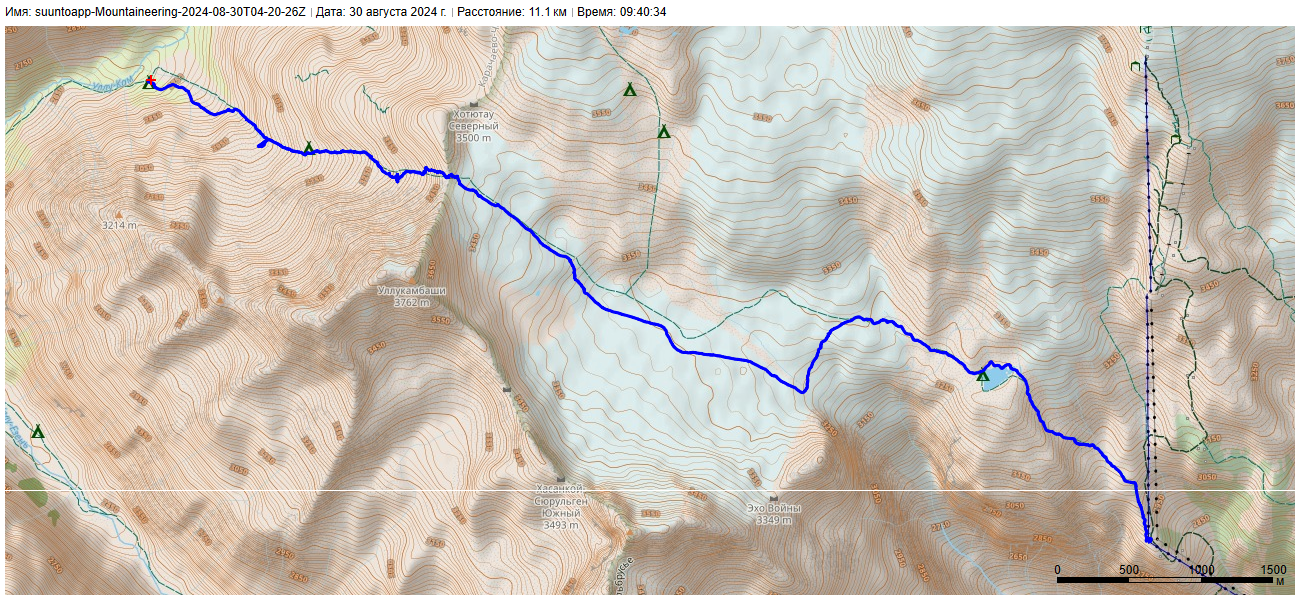
\includegraphics[angle=0, width=0.7\linewidth]{../pics/mini_maps/30}
	\label{fig:mini_30}
\end{figure}





Мы проснулись утром рано в 05:30. Позавтракали двойной порцией сухого омлета и отправились в путь в 07:20.

\begin{figure}[h!]
	\centering
	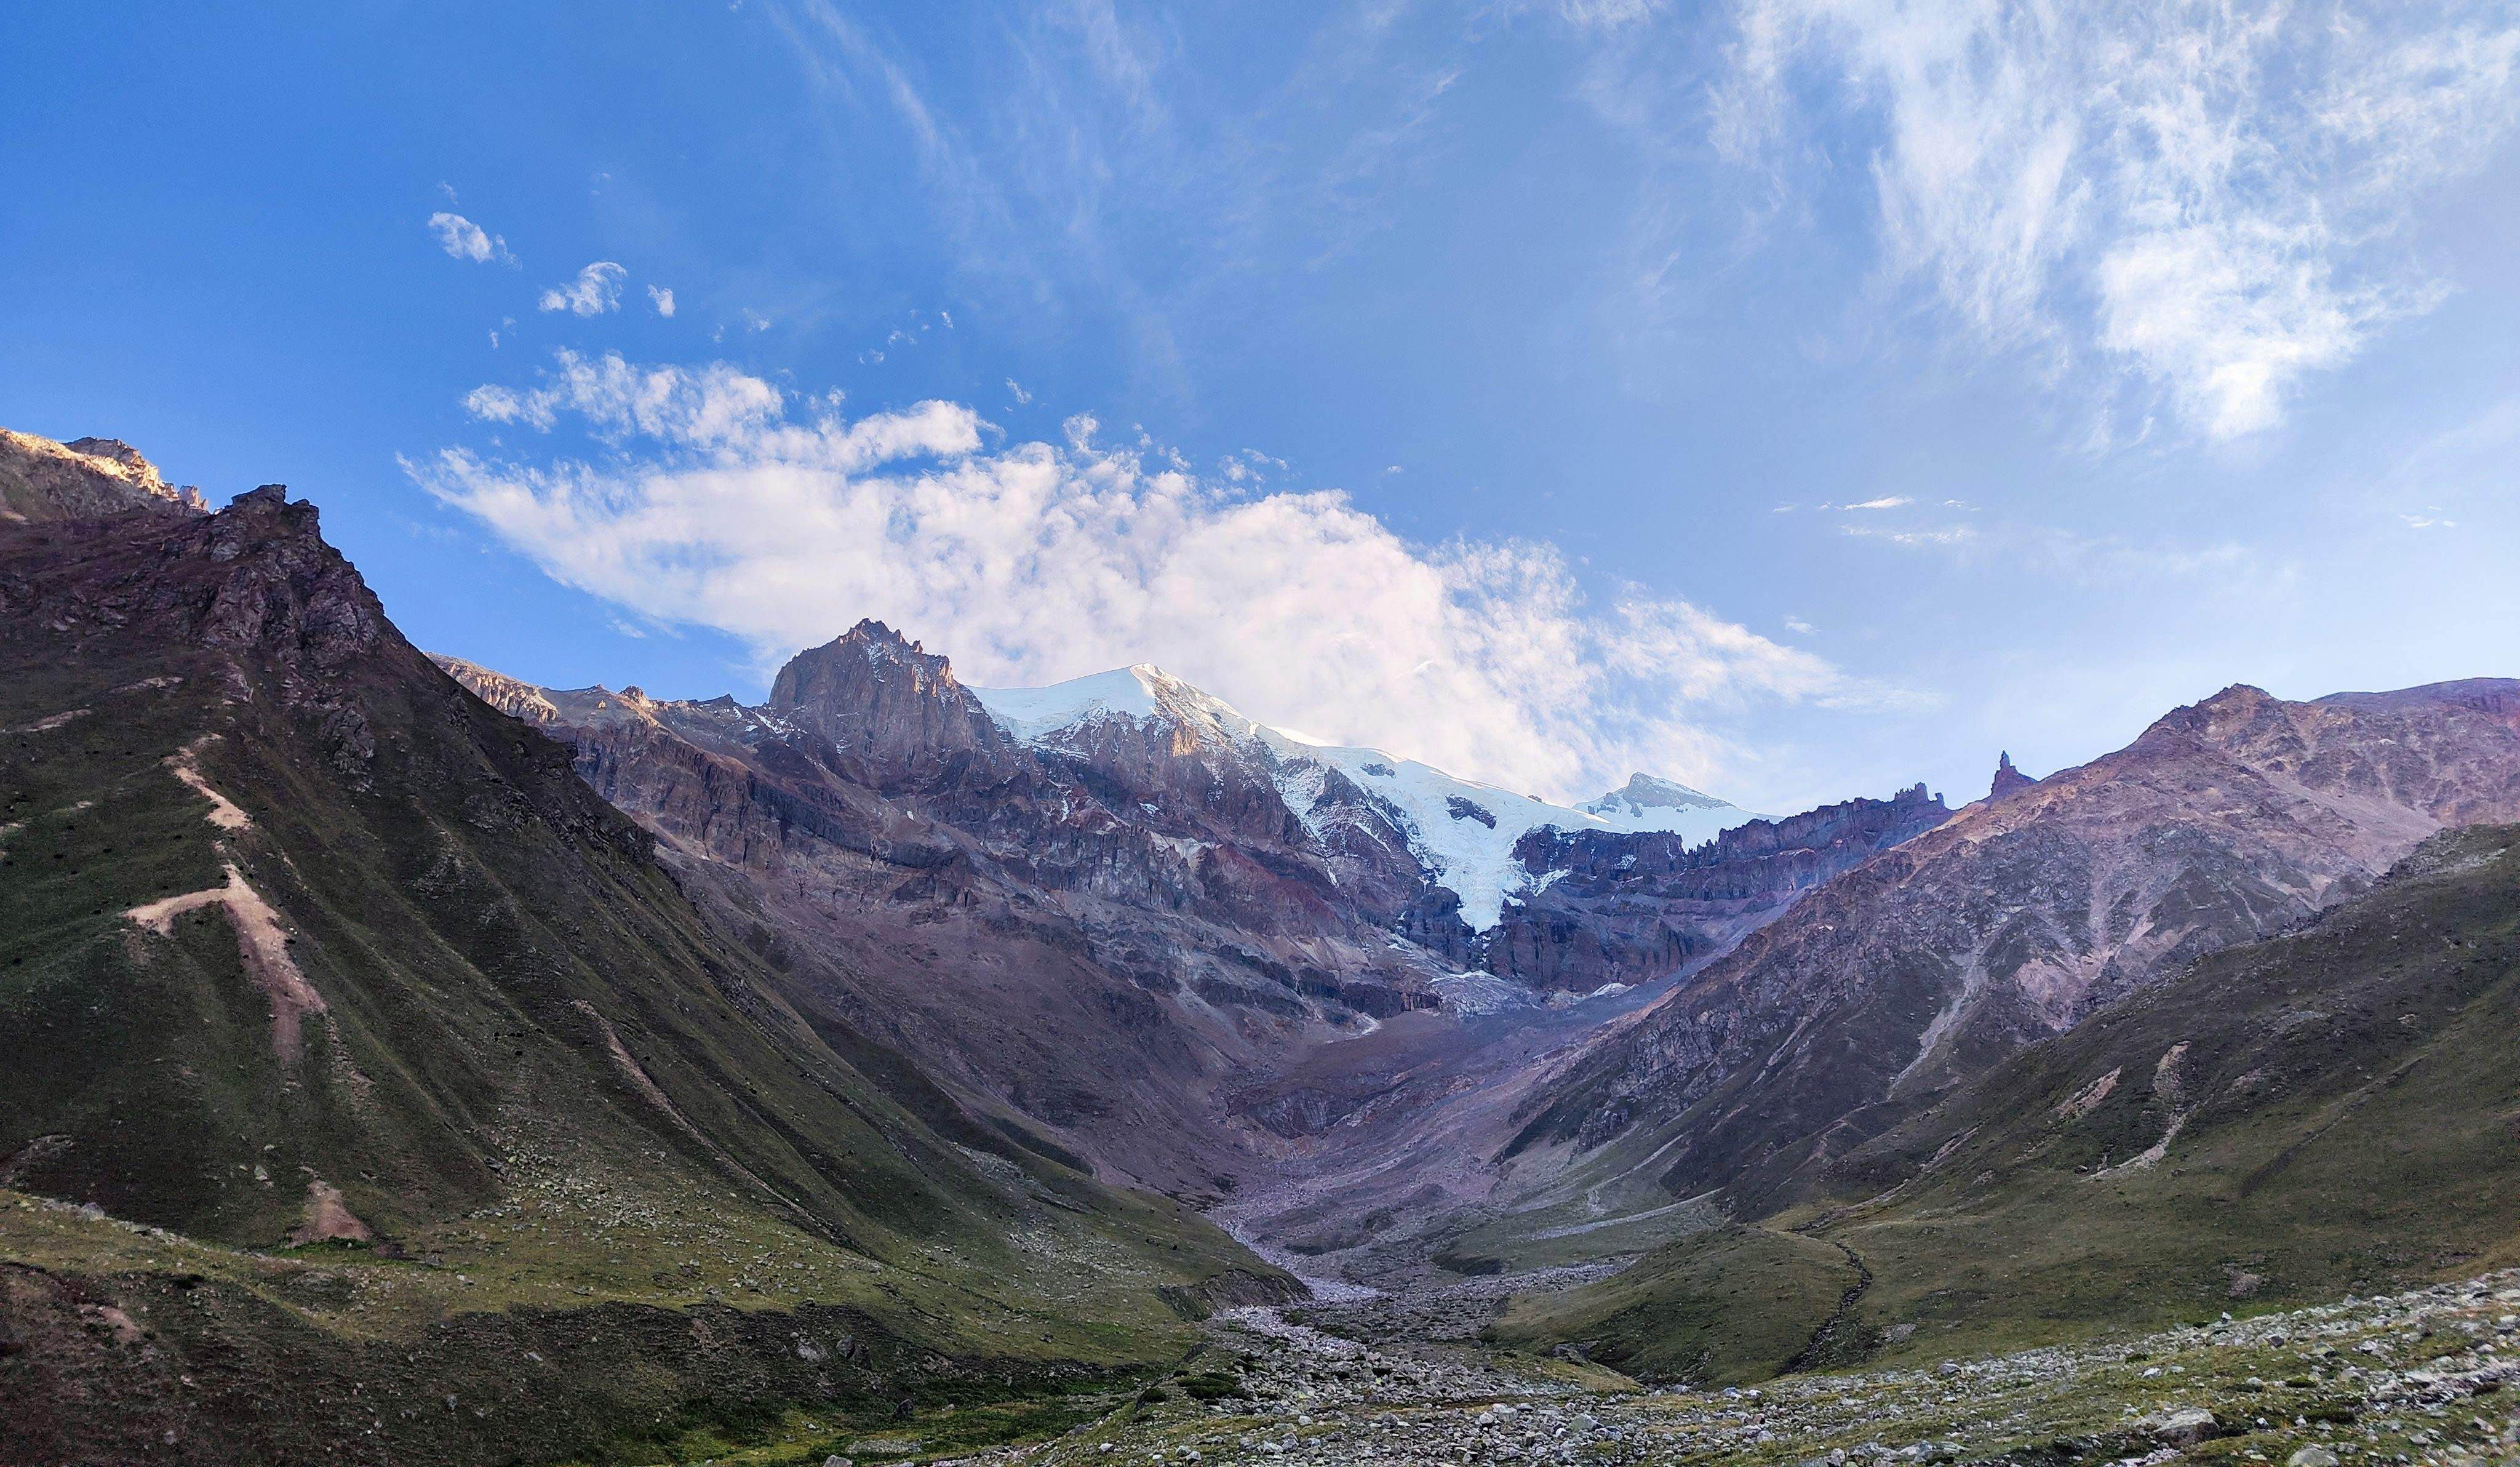
\includegraphics[width=0.7\linewidth]{../pics/IMG_20240830_063548}
	\caption{Утренний вид на юго-западные склоны Эльбруса}
	\label{fig:IMG_20240830_063548}
\end{figure}

До перевала ползли без особых проблем~--- сыпуха и курумник к концу похода стали нам родными и знакомыми. Путь технически и физически не сложный, но морально несколько утомляет, так как необходимо набрать 800 м высоты. Огромной поддержкой оказались синие метки трека для трейлраннеров Alpindustria Elbrus Race. Они значительно сократили нам время на поиск пути.

\begin{figure}[h!]
	\centering
	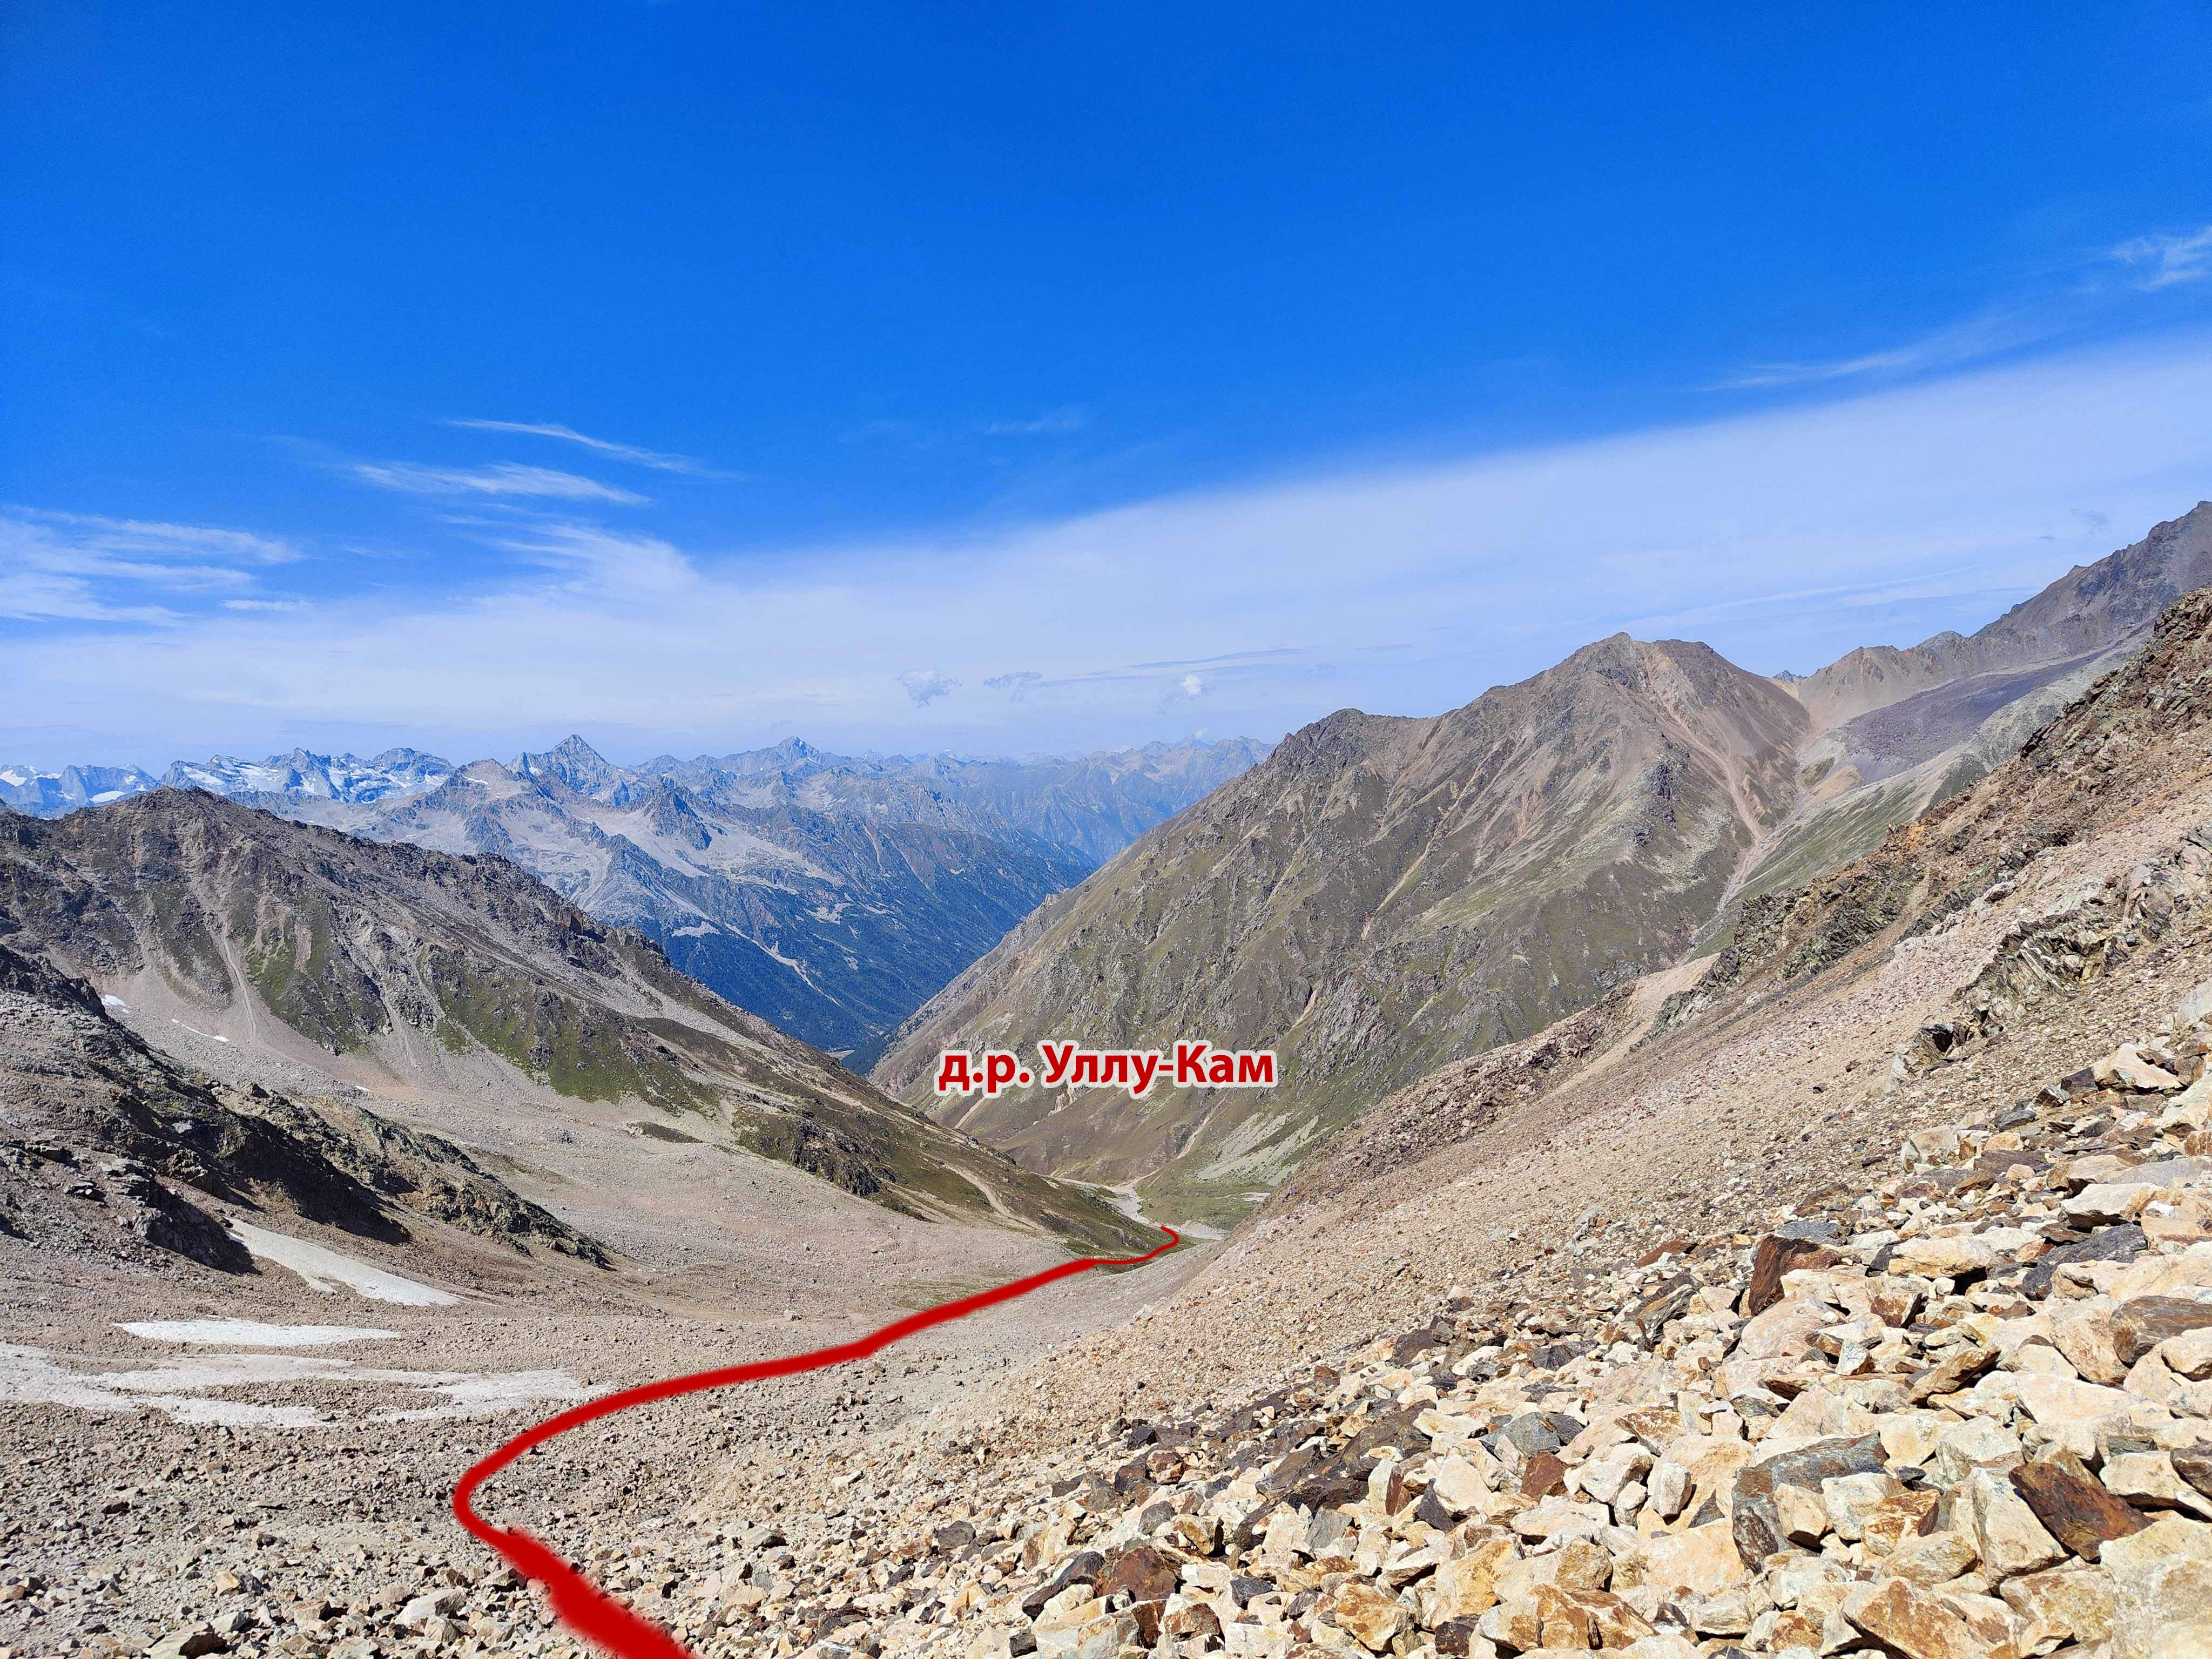
\includegraphics[width=0.7\linewidth]{../pics/IMG_20240830_105443}
	\caption{Вид на путь подъёма}
	\label{fig:IMG_20240830_105443}
\end{figure}

\begin{figure}[h!]
	\centering
	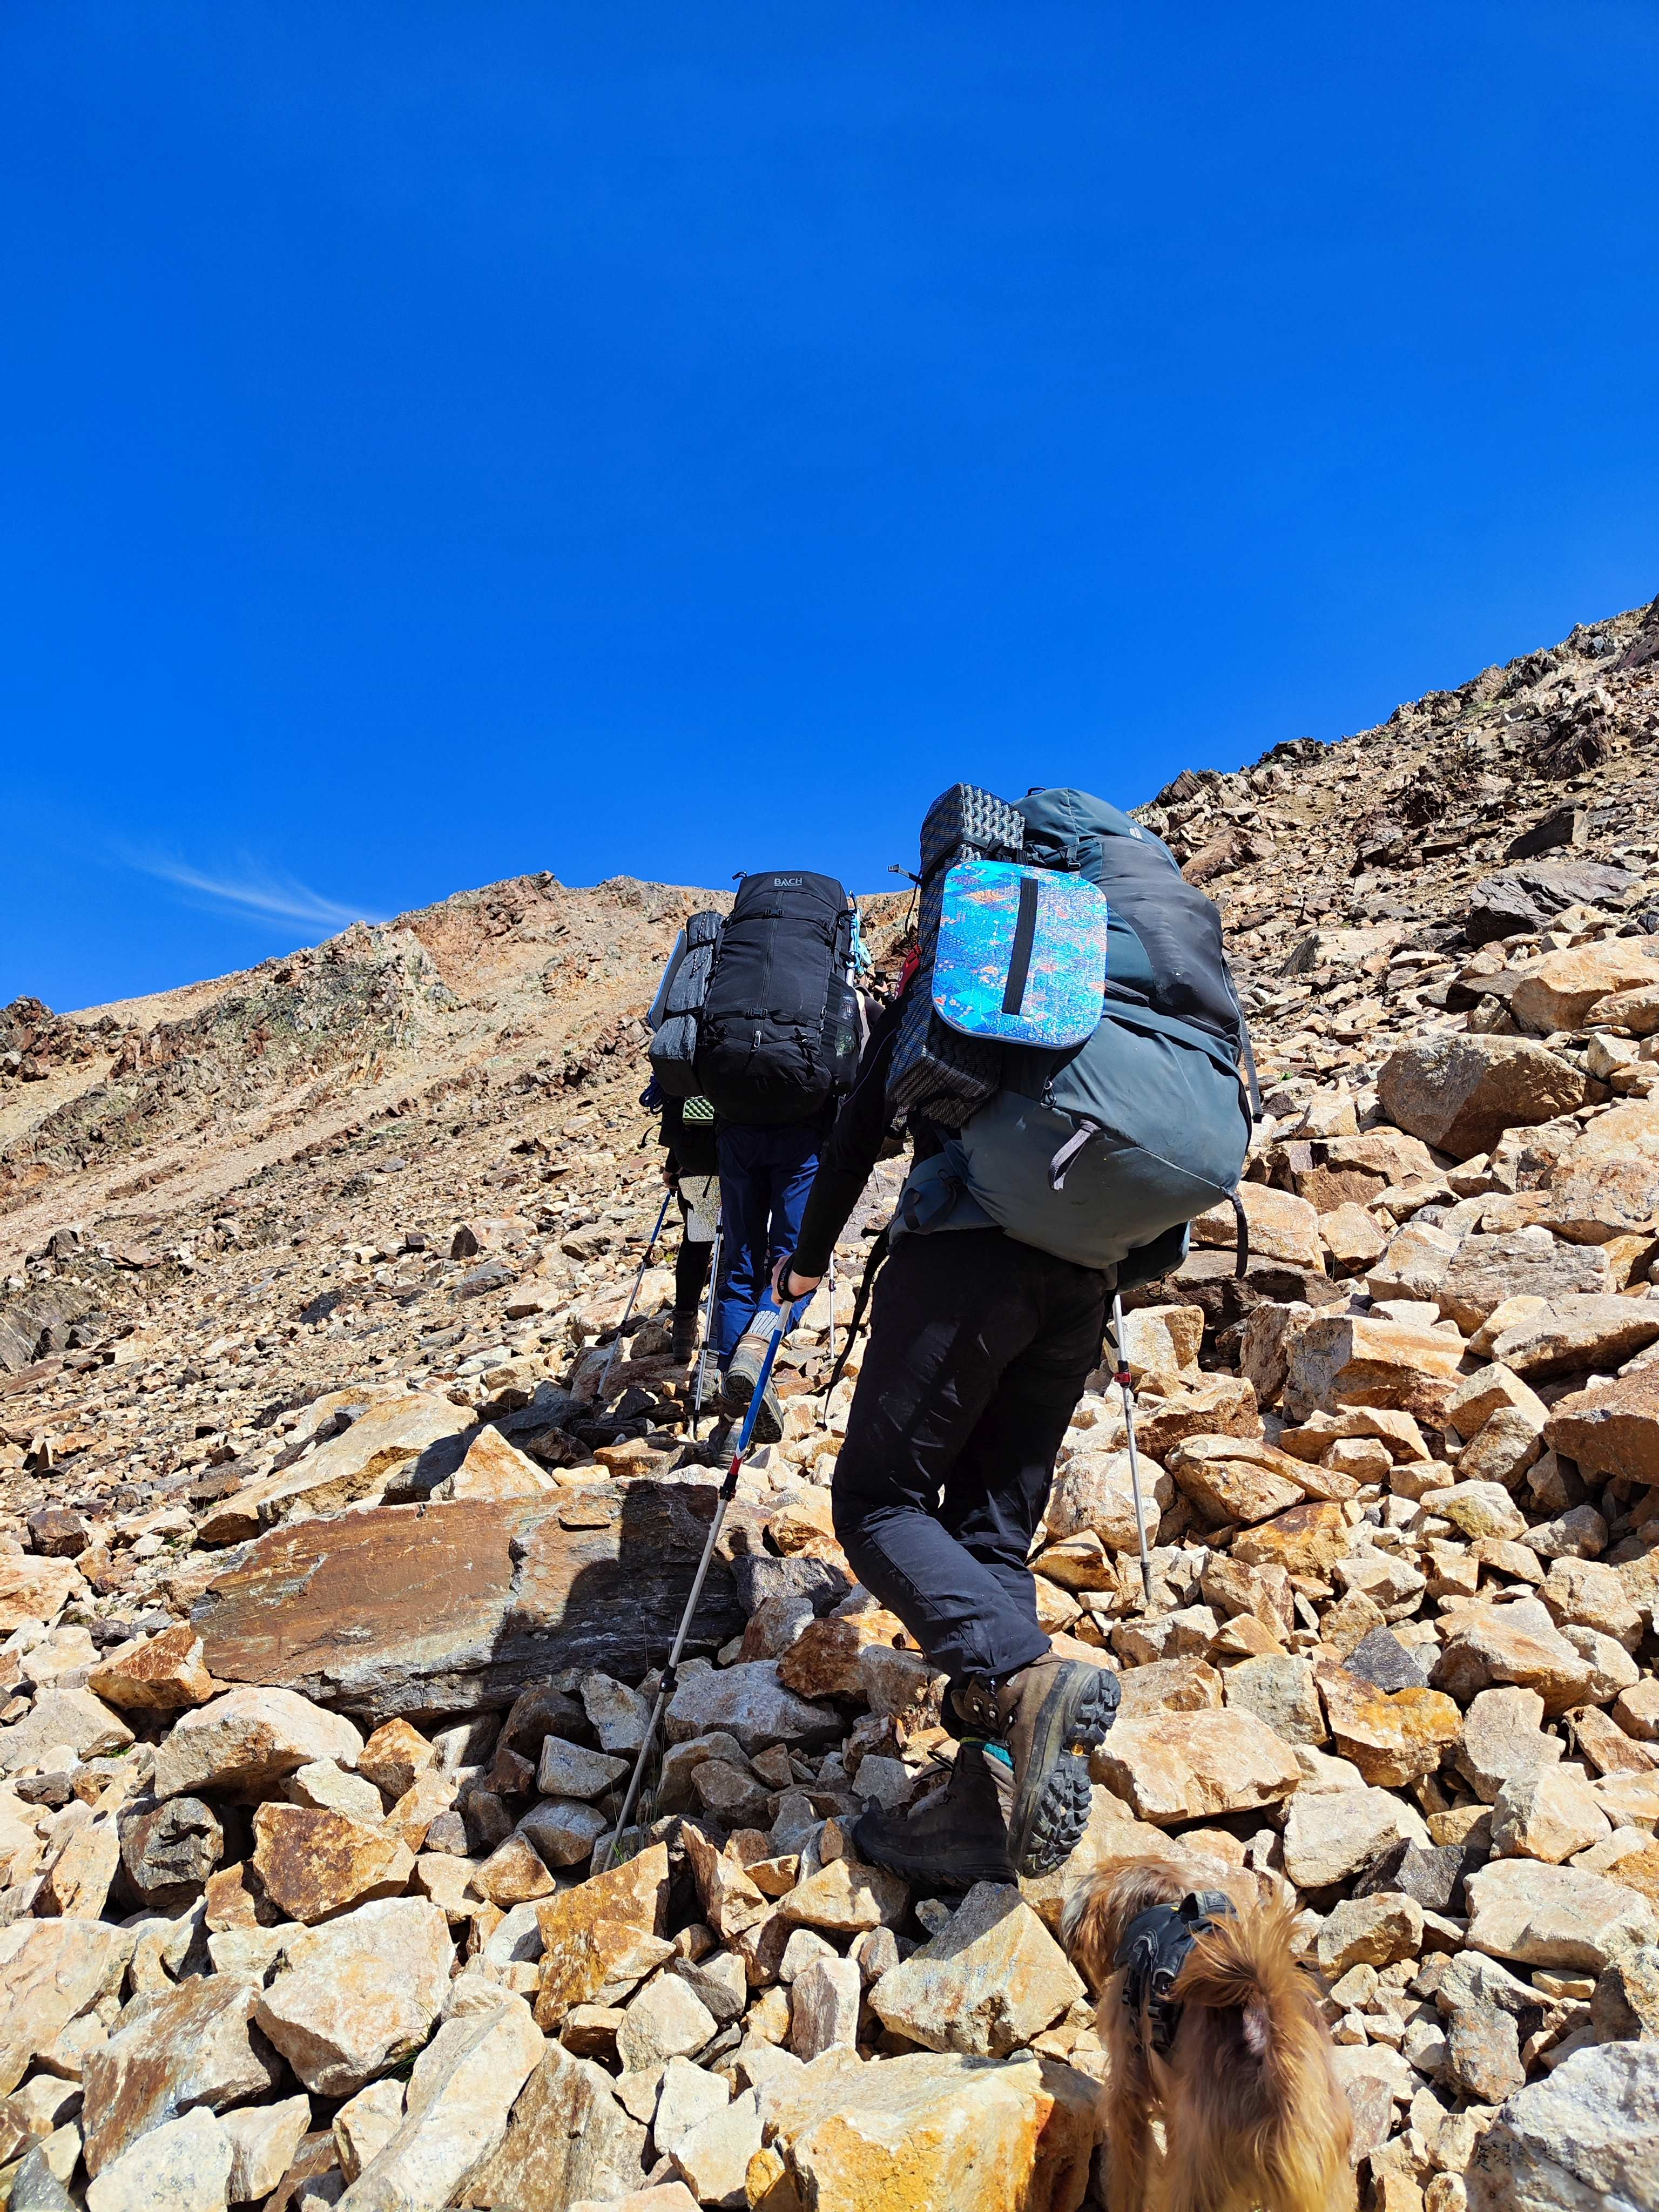
\includegraphics[width=0.7\linewidth]{../pics/IMG_20240830_105447}
	\caption{Поднимаемся на перевал}
	\label{fig:IMG_20240830_105447}
\end{figure}

\begin{figure}[h!]
	\centering
	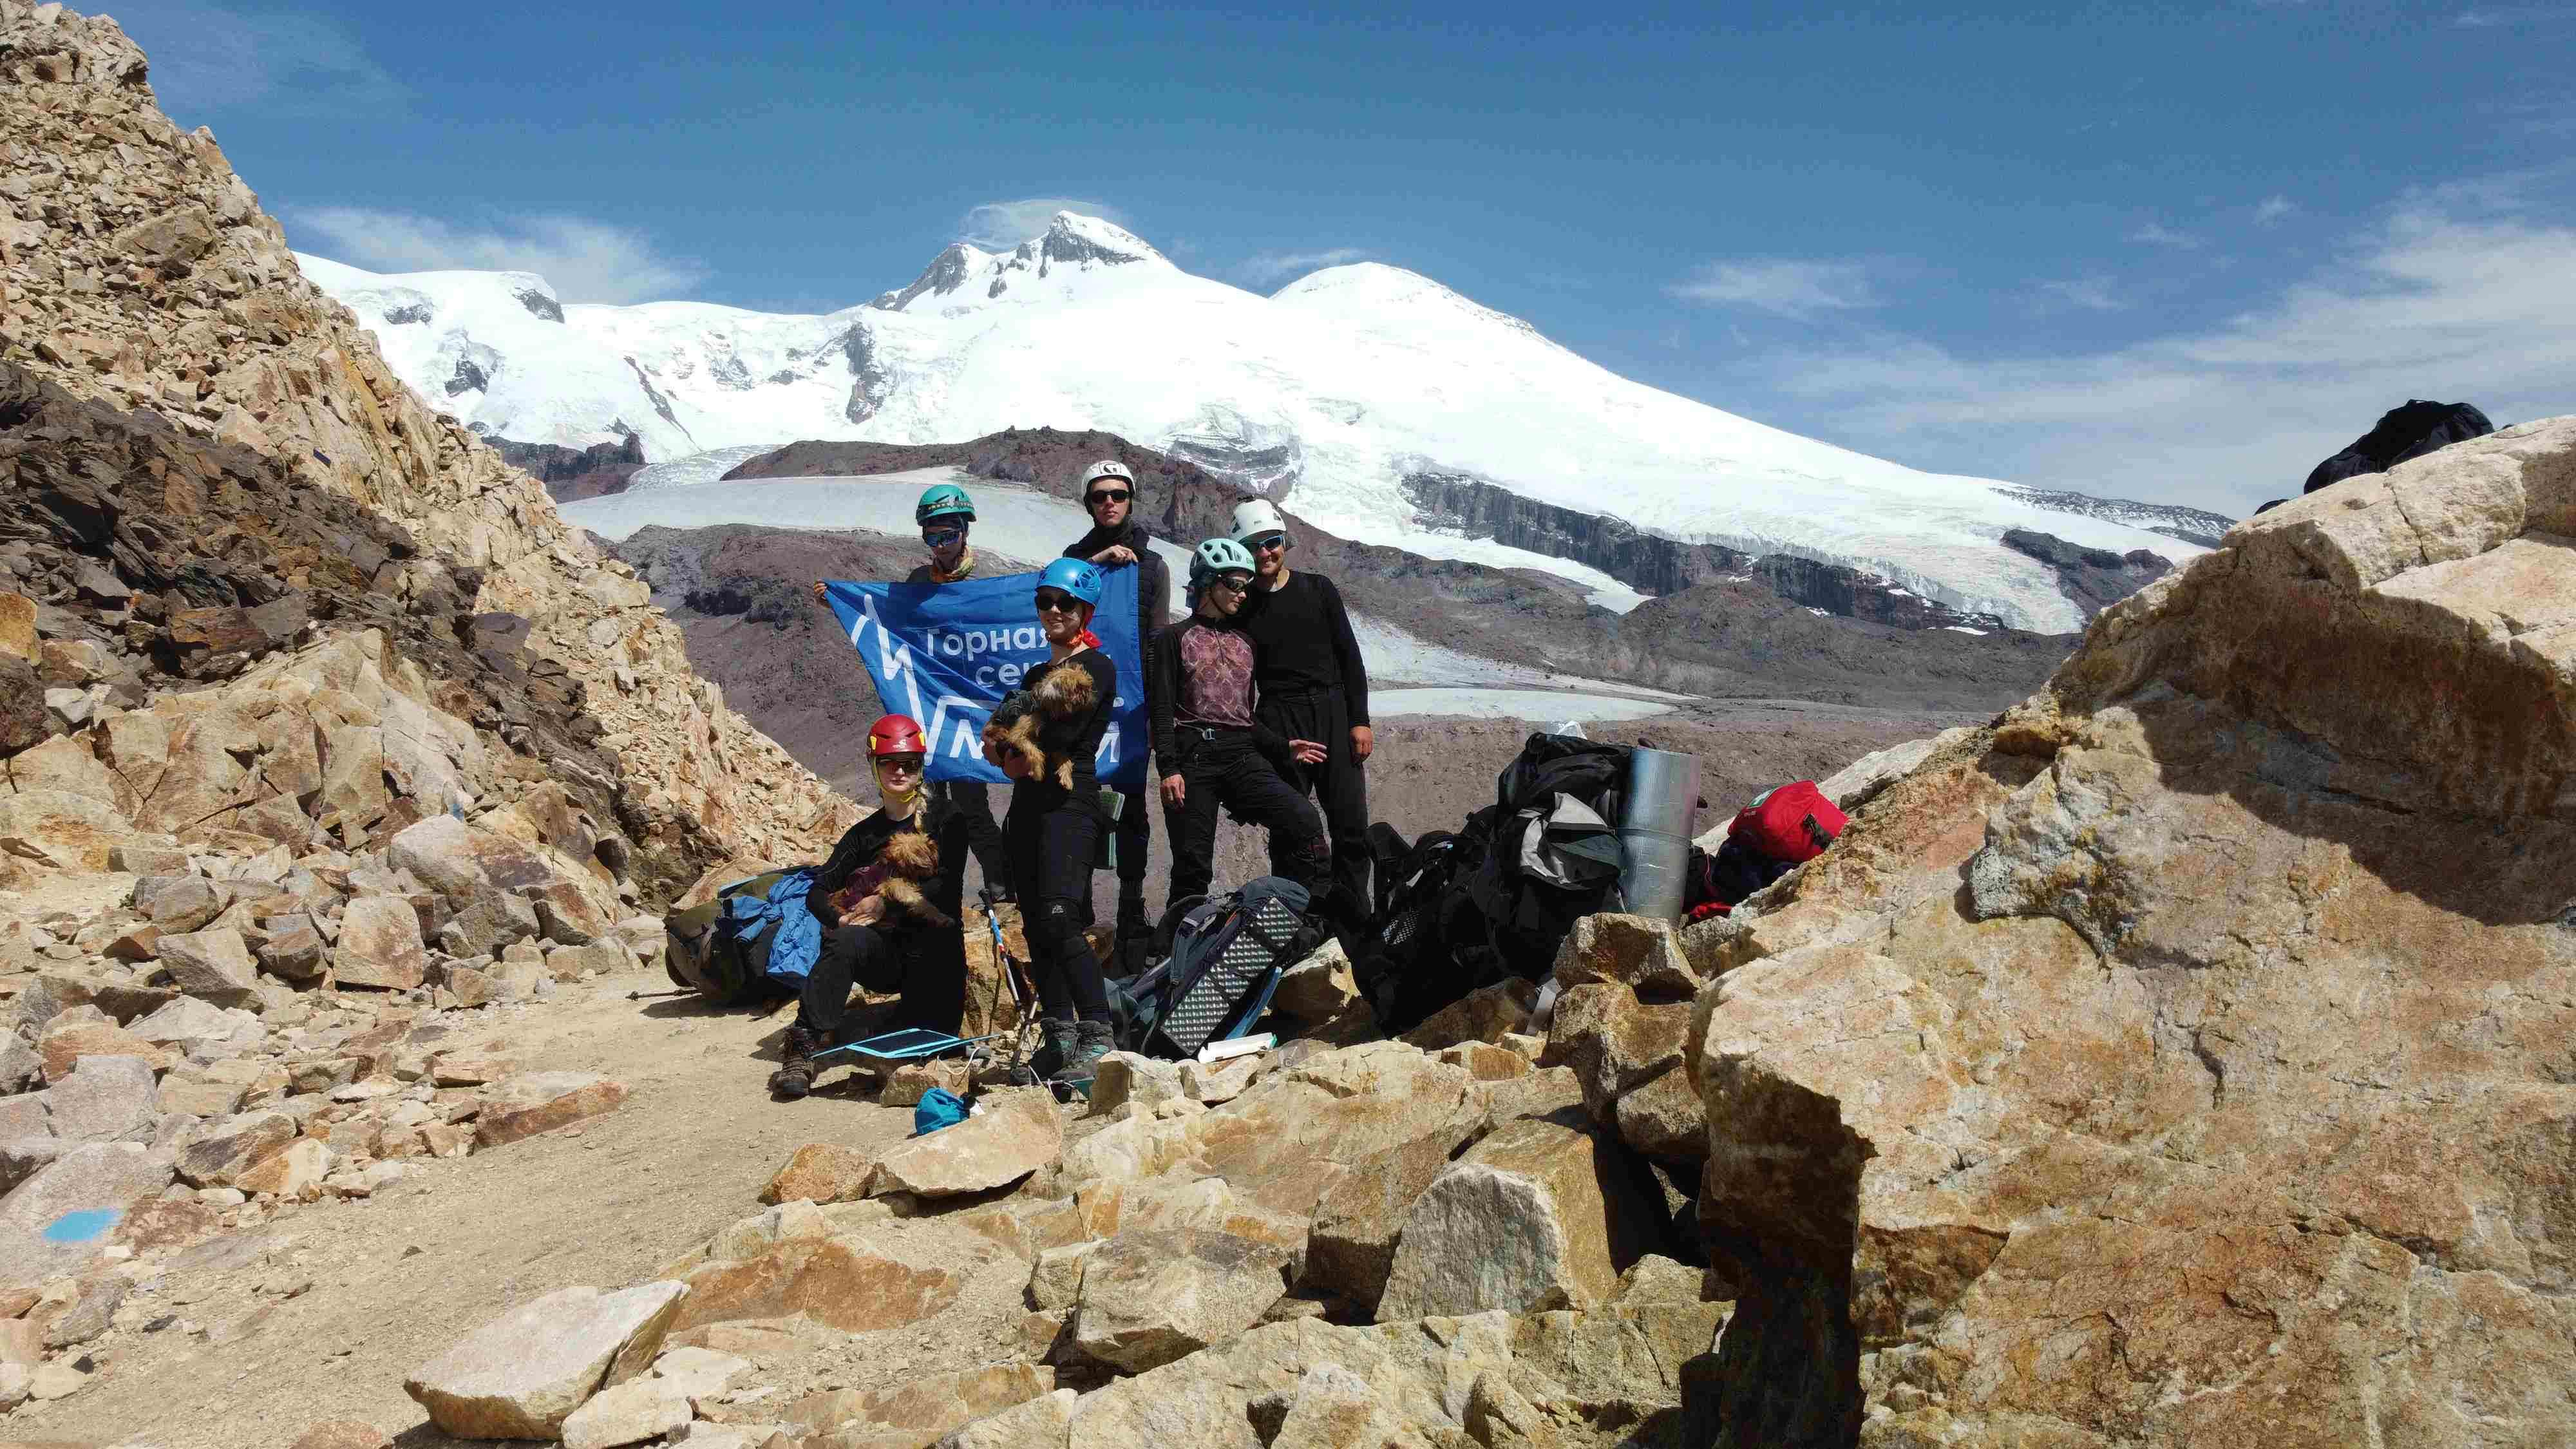
\includegraphics[width=0.7\linewidth]{../pics/DJI_0899}
	\caption{группа на пер. Хотютау}
	\label{fig:hotyutau_1}
\end{figure}

В .. взошли на перевал. Полюбовались Эльбрусом, обломками вертолета на его склоне и букетом памятных табличек на самом перевале. Сняли записку проекта "Виртуальные горы" от 28.08.2024 и турклуба "ЛИИЖТ" г. Санкт - Петербург от 21.08.2024.

В .. начали спуск с перевала. Спуск по песчаному склону неприятный, но быстрый. В .. (N, E) надели кошки, подвязались блокировкой и начали движение по леднику. Ледник был открытый, трещины хорошо просматривались и легко обходились.

*Вставить фотографию собачек в ботиночках*

Через несколько минут нас нагнала группа из двху человек из горной секции МАИ. Как выяснилось, оставленная нами записка пролежала в камнях не более получаса :) Увеличенным составом мы двигаемся по леднику до начала ледопада, где подро сворачиваем налево и плутаем в обачном тумане, пока зоркий глаз не выцепляет вдалеке знокмую синюю метку. По портоптанной дорожке далее едем без проблем. 

В .. выходим к Эльбрусскому озеру. В этот момент выясняется, что до закрытия канатной дороги остается меньше получаса. Остаток пути идём на всех парах и садимся в кабинку в 17:00 ровно. Спустившись в поляну Азау, оплачиваем безбилетный проезд в закрытой , но приоткрывшейся специально для нас кассе. На этом мы прощаемся с нашими новыми друзьями и горная часть нашего путешествия завершается.

Хорошо проводим время в заведении "не помню". В 20:00 нас встречает микроавтобус и везет нас до вокзала "не помню" где мы встречаемся с частью слившихся участников. После полуночи загружаемся в поезд и катим домой!!!







\clearpage